\documentclass[twocolumn]{article}
\setlength{\columnsep}{20pt}
%\usepackage{url}
%\usepackage{algorithmic}
\usepackage[a4paper]{geometry}
\usepackage{datetime}
\usepackage[font=small,labelfont=it]{caption}
\usepackage{graphicx}
% Use Times NR as font
\usepackage{lmodern}
\usepackage[T1]{fontenc}

\usepackage{float}

% Better tables
\usepackage{tabularx}
% to make beautiful tables
\usepackage{booktabs}

\usepackage{microtype}
\usepackage{amsmath}
\usepackage{subfigure}

% Letterspacing macros
\newcommand{\spacecaps}[1]{\textls[200]{\MakeUppercase{#1}}}
\newcommand{\spacesc}[1]{\textls[50]{\textsc{\MakeLowercase{#1}}}}

\title{\huge{\textbf{Study doc: margin experiment}}\\ \normalsize \Large{how does the margin affect the embedding space}}

\author{Fabian Gröger\\fabian.groeger@stud.hslu.ch}
\date{\today}

\begin{document}
\maketitle

\begin{abstract}
This experiment aims to show the affect of changing the margin $\alpha$ within a triplet loss on the DCASE dataset.
\end{abstract}


\section{Introduction}
A very important hyperparameter when training a triplet loss is the margin, denoted as $\alpha$. The margin makes sure that the network is not allowed to output the trivial solution, where all the embeddings vectors are zero or contain the same values. Within the triplet loss function, it is used to put a limit on how far the network can push the negative sample away to improve the loss. Thus the distance of the negative sample has to be higher than the distance from the anchor to the positive sample plus the margin $\alpha$. This experiment aims to show the importance of the margin as well as to find the optimal one for the DCASE dataset.

\section{Hyperparameters}
The hyperparameters used for this experiment are shown in table \ref{tab:Hyperparameters}. The margin will be evaluated using a state of the art ResNet18 architecture on the DCASE dataset. The hyperparameters in section \textit{Feature representation} as well as the sample rate are the default ones proposed by the organisers of the DCASE challenge within the baseline project. The margin will be evaluated for six different values \texttt{[0.3, 0.5, 0.7, 1, 2, 10]}.

\begin{table}[H]
    \centering
    \caption{Hyperparameters used for the experiment}
	\label{tab:Hyperparameters}
    \begin{tabular}{l|l}
        \toprule
        \textbf{Hyperparameter} & \textbf{value} \\ 
        \midrule[1pt]
        Dataset & DCASE \\
        \hline
        Model & ResNet18 \\ 
        \hline
        Epochs & 10 \\ 
        \hline
        Batch size & 256 \\ 
        \hline
        Learning rate & 1e-3 \\
        \hline
        Margin & [0.3, 0.5, 0.7, 1, 2, 10] \\
        \hline
        Embedding dimension & 512 \\
        \hline
        Prefetch batches & 2048 \\ 
        \hline
        Random selection buffer & 64 \\ 
        \hline
        Shuffle dataset & True \\
        \midrule[1pt]
        \multicolumn{2}{l}{\textit{Multi threading}} \\
        \midrule[1pt]
        Number of generators & 16 \\ 
        \hline
        Number of parallel calls & 16 \\
        \midrule[1pt]
        \multicolumn{2}{l}{\textit{Audio sample}} \\
        \midrule[1pt]
        Sample rate & 16000 \\ 
        \hline
        Sample size & 10 \\
        \hline
        Sample tile size & 2 \\
        \hline
        Sample tile range & 4 \\
        \hline
        Convert to mono & True \\
        \midrule[1pt]
        \multicolumn{2}{l}{\textit{Feature representation}} \\
        \midrule[1pt]
        Feature extractor & LogMelExtractor \\ 
        \hline
        Frame length & 480 \\
        \hline
        Frame step & 160 \\
        \hline
        FFT size & 1024 \\
        \hline
        Number of Mel bins & 128 \\
        \hline
        Number of MFCC bins & 13 \\
        \bottomrule
    \end{tabular}
\end{table}

\begin{figure}[t]
\centering
    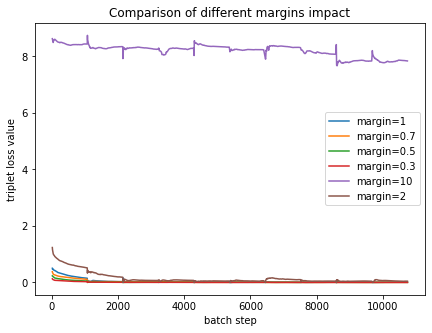
\includegraphics[width=\linewidth]{assets/margin_all_plot.png}
    \caption{Plot of the triplet loss value of all margins}
    \label{fig:margin-all}
\end{figure}

\section{Results}

Five models with the same hyperparameters, shown in table \ref{tab:Hyperparameters}, were trained for ten epochs. The value of the triplet loss is the most important criteria for selecting the optimal margin since the margin has the most significant impact on the loss function. Figure \ref{fig:margin-all} shows all the trained models in a single plot to visualise the impact on changing the margin. From this figure, the resulting embeddings improved from the trivial solution as the margin is increased. Thus as the margin is decreased the total number of triplets generated whose loss is higher than zero decreases, therefore, they do not contribute to the training of the model thus reducing the accuracy of the outputted embedding’s.

There is a vast difference in the value of the loss values. The \texttt{margin=10} has by far the highest loss value of approximately 8, which is very intuitive since the distance to the opposite has to be higher than the distance to the neighbour plus the margin, which is in this case \texttt{8}. This constraint is tough to satisfy, and therefore the loss is relatively high.

The smallest loss value is the one from the \texttt{margin=0.3}. The reason for that is the same as for the high margin, but vice-versa. The constraint it has to satisfy is that the distance to the opposite has to be higher than the distance to the neighbour plus the margin. This is very easily satisfied since it is a relatively small distance.

The figure \ref{fig:margin-5-7-10} shows the triplet loss of the margin values \texttt{0.5, 0.7, 1.0}. It can be seen that the loss is fairly similar and approaches zero.

\begin{figure}[t]
\centering
    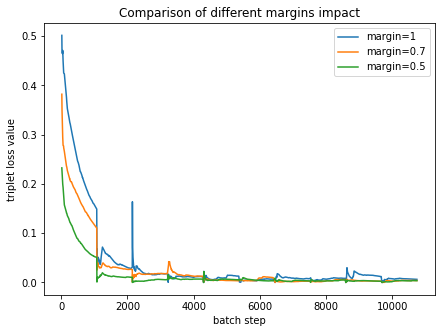
\includegraphics[width=\linewidth]{assets/margin_5_7_10_plot.png}
    \caption{Plot of the triplet loss value of the margins=\texttt{0.5, 0.7, 1.0}}
    \label{fig:margin-5-7-10}
\end{figure}

\section{Conclusion}
Since the highest and lowest margin can be omitted simply by examining the triplet loss plot because the lowest margin does not contribute to the training and the highest sets a constraint which can only be satisfied in a small number of cases, in the other cases it is a much harder decision since the loss value is fairly the same. However, when looking at the resulting embedding space, it can be seen that the \texttt{margin=1.0} distances between the centroids of each label are fairly equally distributed, which is the optimal outcome. Figure \ref{fig:dist-margin-1} shows the distance matrix of the \texttt{margin=1.0}. Whereas the other margins do not have such an equally distributed distance matrix, which indicates that one or more label can be distinguished better than others. However, the optimal solution should be that the distances from all clusters are fairly the same. Therefore the \texttt{margin=1.0} is chosen as the optimal parameter for the DCASE dataset and will be used in all of the further experiments as the standard hyperparameter.

\begin{figure}[t]
\centering
    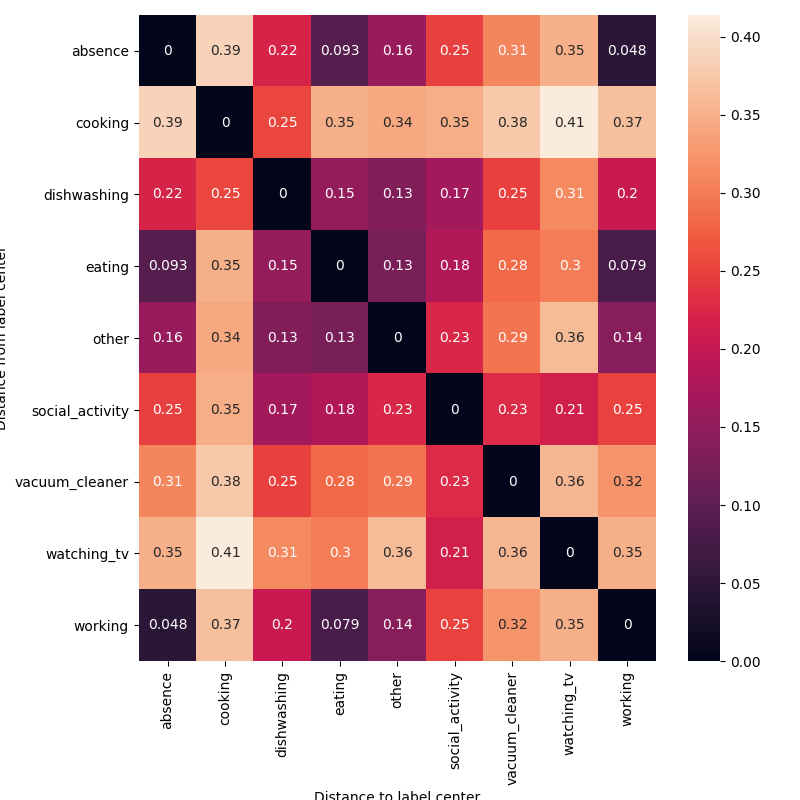
\includegraphics[width=\linewidth]{assets/distance_mat_margin_1.png}
    \caption{Distance matrix of the margin=\texttt{1.0}}
    \label{fig:dist-margin-1}
\end{figure}

\section{Next steps}
This experiment has to be also conducted for the music dataset since this parameter is heavily depended on the used dataset. The margin can be evaluated again when the final audio representation as well as the final model is defined. It should be further fine tuned in the final setting.

\end{document}